% !TEX root = ../main.tex
\chapter{Proof of Concept}\label{ch:PoC}
In this section, we describe the proof-of-concept implementation to calculate the metrics of the model, which can be found publicly in GitHub \footnote{\url{https://github.com/NuriaBruchTarrega/alexandria}}. In order to empirically validate the metrics defined in the previous section, it is necessary to be able to calculate them. Therefore, we decided to create a proof-of-concept tool to calculate the metrics for real-world libraries, and be able to experiment with the results. First, we discuss the possible techniques to implement it and describe the chosen one. Then, there is an explanation of how each metric is calculated, including pseudo-code, to illustrate it.

\section{Analysis technique}
Several techniques could have been used to implement the PoC that calculates the different metrics proposed.

\begin{itemize}
  \item Bytecode analysis
  \item Source code analysis
  \item Call-level dependency graph
\end{itemize}

After an initial effort, source code analysis has been discarded. The reason for it is that the source code is needed for both the client library and all its dependencies. Although it is sometimes available in Maven, it is not available as often as the bytecode. Furthermore, obtaining the code from GitHub created issues when resolving the dependency tree, since in many cases, the version of the dependency being used in the repository, was not yet available in Maven. Therefore, the dependency tree could not be resolved.

The option of call-level dependency graphs is useful for the metrics that measure method invocations. However, the information needed to calculate aggregation coupling is not contained in the call-level graphs. Therefore, the approach to develop this PoC has been bytecode analysis. Furthermore, obtaining the complete dependency tree's call-graphs is still a work in progress within the FASTEN project \footnote{\url{https://www.fasten-project.eu/}}.

\subsection{Bytecode analysis}
The model proposed in this research is meant to be language-agnostic. Nevertheless, the proof-of-concept scope is limited to Java, since the bytecode analysis performed by the proof-of-concept is limited to this programming language. Furthermore, the PoC is focused on the libraries available in Maven. It has been decided to limit the scope to Java and Maven, since it allows to compare the results with the research by Soto-Valero et al. \cite{soto2020comprehensive} (see Section \ref{sec:Exp1}). Furthermore, the work done by the FASTEN project, is also focused in Maven, and therefore it will be easier in the future to compare the results when measuring the metrics with byte-code analysis and call-graphs, since the source will be the same.

\subsubsection{Architecture}

The proof-of-concept tool is divided into two parts: the frontend and the backend. The frontend contains the visualizations proposed to see the dependency tree and display the metrics of the model. Meanwhile, the backend receives requests to calculate the dependency tree for a given Maven library. The response to a request consists of the result of the calculation of the metrics for each server library in the dependency tree of the given client library.
The implementation of the backend is supported by the libraries  \textit{Aether}\footnote{\url{https://wiki.eclipse.org/Aether/What_Is_Aether}}, and \textit{Javassist}\footnote{\url{http://www.javassist.org/}}.

\paragraph{Aether}
Aether is a library created by Eclipse, which allows us to fetch Maven artifacts from different repositories. Besides, it is also used to resolve the dependencies of a library and create the dependency tree. To create the dependency tree, Aether uses the same strategy to resolve the dependencies as Maven.

In the PoC, this library has been used for the initial steps. The request to calculate the metrics receives the identifiers of the library to analyze (\textit{GroupId}, \textit{ArtifactId}, and \textit{version}). Aether is used to fetch the library \textit{jar} and \textit{POM} files from the Maven Central Repository.

Once the artifact of the client library is obtained, \textit{Aether} is used to resolve the dependencies of the artifact. For the calculation of the metrics to be possible, all the client library dependencies should also be available in the Maven Central Repository. The dependency tree of the artifact is visited, and each of the dependencies is also obtained to have the \textit{jar} files to analyze. Also, the dependency tree calculated with Aether is used to create a custom dependency tree using the custom class \texttt{DependencyTreeNode}, which stores the data about each of the libraries needed for calculating the metrics. The \texttt{DependencyTreeNode} will be described in greater detail later on.

\paragraph{Javassist}
Javassist is a library that allows the user to perform bytecode manipulation in a simple way. It has two levels, a source-level and a bytecode level. Using the source-code level, it is possible to perform bytecode analysis and manipulation without a deep knowledge of bytecode. Meanwhile, the bytecode level allows the user to manipulate bytecode directly.
For this thesis, the level used is source-code.

The javassist library has been used to interpret and analyze the jars of the client library and all the server libraries. Once the jars of the client library and all its dependencies are available, the first step is to join all the \textit{.class} files in a \texttt{ClassPool} object, which is the main object of \textit{Javassist}. Once the \texttt{ClassPool} is created, it is used to obtain the classes from the client library, from which the different metrics are calculated. The process of calculating the metrics is explained in greater detail in the following.

\paragraph{Overview}

In Figure \ref{fig:overview-backend}, one can see the process the proof-of-concept does to calculate the metrics of the model. First, obtaining the \textit{.jar} files of each library included in the dependency tree. Then, by using \textit{Javassist}, it iterates through the classes of the client library to find the usage of the direct dependencies. Next, based on the direct usage calculated, it iterates through the entire dependency tree to find the necessary data to calculate the metrics of the model. Finally, with all the necessary information stored in the data model, the metrics' value is calculated. The process of obtaining the data to store in the data model and the data model itself are described below.

\begin{figure}[ht!]
\begin{center}
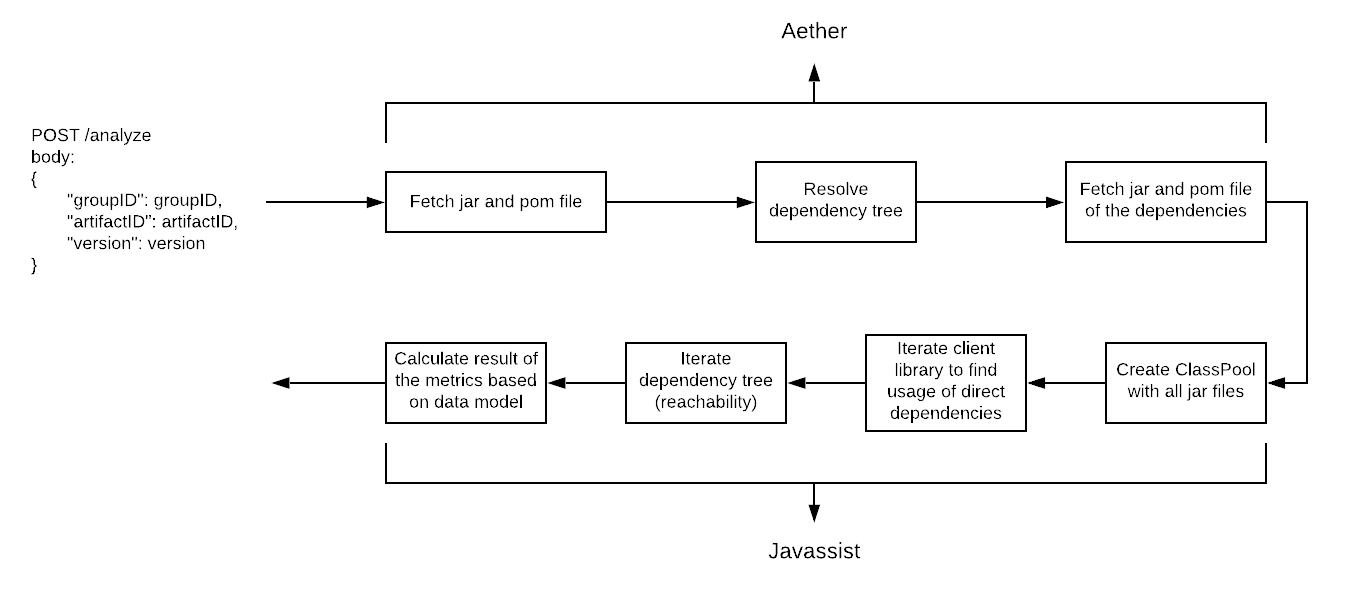
\includegraphics[width=\textwidth]{figures/Overview-Backend.png}
\caption{Overview of the proof-of-concept implementation of the calculation of the model}
\label{fig:overview-backend}
\end{center}
\end{figure}

\subsection{Model of the dependency tree}
In order to represent the dependency tree of the client library, the implementation uses the class \texttt{DependencyTreeNode}. Each \texttt{DependencyTreeNode} contains the information of the library it represents, namely \textit{groupID}, \textit{artifactID}, and \textit{version}. Also, to represent the dependencies of the library represented by each  \texttt{DependencyTreeNode}, there is a \texttt{List} of \texttt{DependencyTreeNode}.

To store the information needed to calculate the coupling metrics, there are two other classes: \texttt{MicBehaviors}, \texttt{AcClasses}, for \texttt{MIC} and \texttt{AC} respectively. \texttt{MicBehaviors} is a map, containing for each method or constructor (behavior) of the server library used to calculate \texttt{MIC}, a \texttt{Set} with all the method calls from which it is reachable. In the same way, \texttt{AcClasses} is a map, in which for each class of a server library used to calculate \texttt{AC}, there is a \texttt{Set} of all the field declarations from which the class is reachable. The behaviors and classes used to calculate \texttt{MIC} and \texttt{AC} are those which are reachable through the type of connection of the metric.

Each \texttt{DependencyTreeNode} has an object \texttt{MicBehaviors} and \texttt{AcClasses} for each of the distances at which the metric is measured, stored as a map, where the distance is the key and \texttt{MicBehaviors} or \texttt{AcClasses}, the value.

Also, for the metrics that measure the dependencies' coverage, two additional fields have been created: \texttt{ReachableClasses} and \texttt{ReachableBehaviors}. The first field is to calculate the \texttt{\%ReachableClasses}, and the second one for \texttt{\%ReachableMethods}. Both \texttt{ReachableClasses} and \texttt{ReachableBehaviors} are sets containing the classes, in the first case, and behaviors in the second case, of the library represented by the \texttt{DependencyTreeNode}, which are reachable from the client library.

\begin{figure}[ht!]
\begin{center}
\includegraphics[width=\textwidth]{figures/Thesis-ModelClassDiagram.png}
\caption{Class diagram, dependency tree model}
\label{fig:class-diagram-tree}
\end{center}
\end{figure}


\section{Calculating coupling metrics}
This section contains the description of how the metrics \texttt{MIC}, \texttt{AC}, \texttt{TMIC}, and \texttt{TAC} are calculated in the implementation of the PoC. During this section, we use the terminology of the library Javassist. For example, to refer to methods and constructors, we say behaviors. Also, the classes used from Javassist are named as \texttt{Ct<name of the element>}, where \texttt{Ct} means compile-time. Therefore, the class representing a java class is \texttt{CtClass}.

\subsection{Method Invocation Coupling}
The pseudo-code in Figure \ref{fig:algorithm-mic} represents the algorithm used to calculate the metric \textit{MIC} for each one of the direct dependencies of a given client library. The algorithm's output is a map containing the set of \texttt{BehaviorCalls} that call each \texttt{CtBehavior}. The map is generated for each of the direct dependencies and stored in the \texttt{DependencyTreeNode} of each library.

The class \texttt{CtBehavior} contains information about the behavior itself and about the class in which it is declared. Each of the \texttt{CtBehavior} is used later on to find the polymorphic implementations of the behavior and calculate the metrics for the transitive dependencies.

To calculate this first metric, the implementation iterates through all the classes of the client library (line 3). For each class, the behaviors are obtained (line 4).

Then, the tool iterates through all the behaviors (line 5) and calls the method \texttt{instrument}. The main use case of this method is to modify the bytecode of the method, but in this case, we use it to find the connections of interest for this metric. The method \texttt{instrument} receives an \texttt{ExprEditor} object, which is a class that can be extended to implement the methods for editing the bytecode, which are empty by default. To calculate this metric, the overridden methods are \texttt{edit(MethodCall mc)}, \texttt{edit(ConstructorCall cc)}, and \texttt{edit(NewExpr ne)}. These methods will be called for each method call or constructor call, existing in the method (line 6). The constructor calls in the form of \texttt{this()} or \texttt{super()} are captured by the method \texttt{edit(ConstructorCall cc)}. Meanwhile, the constructor calls in the form of \texttt{new Object()} are captured by \texttt{edit(NewExpr ne)}.

Each captured call to a behavior is checked if the called behavior belongs to a server library (line 9). In case it does, the call is added to the \texttt{MicBehaviors} map of the server library (line 10), with 1 as the distance at which the connection is found since it is a direct dependency.

\begin{figure}[ht!]
\begin{lstlisting}[escapeinside={(*}{*)}]
clientClasses = classPoolManager.getClientLibraryClasses()

for each clientClass in clientClasses
  behaviors = clientClass.getDeclaredBehaviors()
  for each behavior in behaviors
    for each behaviorCall in behavior
      serverBehavior = behaviorCall.getBehavior()
      serverClass = serverBehavior.getDeclaringClass()
      if (classPoolManager.belongsToDependency(serverClass))
        dependencyTreeNode.addMicBehavior(serverBehavior, behaviorCall, distance = 1)
\end{lstlisting}
\caption{Pseudo-code of the algorithm to calculate MIC}
\label{fig:algorithm-mic}
\end{figure}

\subsection{Aggregation Coupling}
The pseudo-code in Figure \ref{fig:algorithm-ac} represents the algorithm used to calculate the metric \texttt{AC}. The output of the algorithm is a map containing for each \texttt{CtClass} of the server library, the set of \texttt{CtField} that are of the type of the \texttt{CtClass}. The class \texttt{CtClass} represents a class and contains the information about the class itself and about the library where it is implemented. \texttt{CtClass} is used later on to find the descendants of the class and calculate the metric \texttt{TAC} for the transitive dependencies.

The algorithm for this second metric is similar to the previous one. First, the implementation iterates through all the classes of the client library (line 3). Then, for each class, it iterates through all the declared fields (line 5). Next, each of the fields containing a generic type is parsed separately (line 6), to obtain all the types included in the generic (line 7), which are treated individually (line 8). All the simple fields, if the class's implementation is found in a server library (line 13), are included in the calculation of the metric (line 14). The distance is set to 1 due to the server library being a direct dependency.

\begin{figure}[ht!]
\begin{lstlisting}[escapeinside={(*}{*)}]
clientClasses = classPoolManager.getClientLibraryClasses()

for each c in clientClasses
  fields = c.getDeclaredFields()
  for each field in fields
    if (field.containsGeneric())
      serverClasses = getAllClasses(field)
      for each serverClass in serverClasses
        if (classPoolManager.belongsToClientLibrary(serverClass))
          dependencyTreeNode.addAcClass(serverClass, field)
    else
      serverClass = field.getType()
      if (classPoolManager.belongsToDependency(serverClass))
        dependencyTreeNode.addAcClass(serverClass, field, distance = 1)
\end{lstlisting}
\caption{Pseudo-code of the algorithm to calculate AC}
\label{fig:algorithm-ac}
\end{figure}

\paragraph{Inheritance}\label{paragraph:inheritance}
Once the two algorithms (Figures \ref{fig:algorithm-mic} and \ref{fig:algorithm-ac}) are finished, in order to follow the definition of the metrics as specified in section \ref{subsec:metric-definition}, the hierarchies in the server libraries are visited. For the metric \texttt{MIC}, all the polymorphic implementations of the behaviors are found, and for the metric \texttt{AC} all the descendants of the classes.

The algorithms to find the descendants and the polymorphic implementations of the methods are used with each of the libraries with which the client library has a direct dependency, and for which coupling was found, either \texttt{MIC} or \texttt{AC}.

The pseudo-code used to find the polymorphic implementations of the methods can be found in Figure \ref{fig:algorithm-polymorphy}. The process is as follows: First, iterate through all the classes of the server library, given its \texttt{DependencyTreeNode} (line 5). Then, it iterates through the behaviors in the map contained in \texttt{MicBehaviors}. If the current library class is a descendant of the class containing the reachable behavior (line 8) and contains a behavior with the same signature as the reachable behavior (line 9), a polymorphic implementation of the behavior has been found. Therefore, the found behavior is added to the \texttt{MicBehaviors} with the same set of \texttt{BehaviorCall} and distance as the mic behavior (line 11).

\begin{figure}[ht!]
\begin{lstlisting}[escapeinside={(*}{*)}]
serverLibrary = dependencyTreeNode.getLibrary()
micBehaviorsMap = dependencyTreeNode.getMicBehaviors()
serverLibraryClasses = classPoolManager.getLibraryClasses(serverLibrary)

for each serverClass in serverLibraryClasses
  for each micBehavior in micBehaviorsMap
    declaringClass = micBehavior.getDeclaringClass()
    if (serverClass.isSubClassOf(declaringClass))
      if (serverClass.containsBehavior(micBehavior.getSignature()))
        serverBehavior = serverClass.getBehavior(reachableBehavior.getSignature())
        dependencyTreeNode.addMicBehavior(serverBehavior, micBehavior.getBehaviorCalls(), distance)
\end{lstlisting}
\caption{Pseudo-code of the algorithm to find polymorphic implementations}
\label{fig:algorithm-polymorphy}
\end{figure}

The process to find descendants in the case of the metric \texttt{AC} is the same as the one in Figure \ref{fig:algorithm-polymorphy}, but iterating over the \texttt{reachableClassesMap} instead of the \texttt{reachableBehaviorsMap}. Therefore, if the server class is sub-class of a reachable class, it is added to the \texttt{AcClasses} of the library.

\blankl
As can be observed in the previous explanation of how the detection of inheritance is done, in this PoC implementation, it is not detected if a class is extended in the client library instead of in the server library.

\subsection{Transitive Method Invocation Coupling}\label{subsec:tmic}
The calculation of \texttt{TMIC} takes place after calculating \texttt{MIC} for all the direct dependencies of the client library. The methods used in the calculation of \texttt{MIC} from these dependencies are used as a base to calculate \texttt{TMIC}.

To calculate the metric for every dependency in the tree, the dependency tree is traversed using a \textit{breadth-first search (BFS)} on the \texttt{DependencyTreeNode}. The algorithm starts with the direct dependencies since the client library node has already been used for the calculation of \texttt{MIC}. A branch finishes the traversing either when a node does not have more children, or when no reachable methods have been found in a server library. The pseudo-code of the implemented algorithm can be found in Figure \ref{fig:tree-traversing-tmic}.

For each \texttt{DependencyTreeNode} visited, the method \texttt{calculateTransitiveMIC} is executed. The pseudo-code of this method can be found in Figure \ref{fig:calculate-tmic}, which is going to be explained below.

\begin{figure}[ht!]
\begin{lstlisting}[escapeinside={(*}{*)}]
toVisit = queue(clientLibraryNode.getChildren())

while (!toVisit.isEmpty())
  visiting = toVisit.poll()
  if (visiting.hasMicBehaviors())
    findPolymorphicImplementations(visiting.getMicBehaviors())
    if (visiting.hasChildren())
      calculateTransitiveMIC(visiting)
      toVisit.add(visiting.getChildren())
\end{lstlisting}
\caption{Pseudo-code of the \textit{BFS} used for \texttt{TMIC}}
\label{fig:tree-traversing-tmic}
\end{figure}

\begin{figure}[ht!]
\begin{lstlisting}[escapeinside={(*}{*)}]
micBehaviors = visitingTreeNode.getMicBehaviors()

for each micBehavior in micBehaviors
  behaviorsToVisit = queue(micBehavior)
  visitedBehaviors = (*$\emptyset$*)
  while (!behaviorsToVisit.isEmpty())
    visitingBehavior = behaviorsToVisit.poll()
    if (visitedBehaviors.contains(visitingBehavior)) continue
    visitedBehaviors.add(visitingBehavior)

    for each behaviorCall in visitingBehavior
      calledBehavior = behaviorCall.getBehavior()
      calledClass = calledBehavior.getDeclaringClass()
      if (classPoolManager.isStandardClass(calledClass))
        continue
      else if (classPoolManager.isClassInDependency(calledClass, visitingLibrary))
        visitingLibrary.addMicBehaviorToDependency(calledClass, distance + 1)
      else // calledClass is in current library
        behaviorsToVisit.add(calledBehavior)
\end{lstlisting}
\caption{Pseudo-code of the algorithm to calculate \texttt{TMIC}}
\label{fig:calculate-tmic}
\end{figure}

First, we obtain all the behaviors of the visited \texttt{DependencyTreeNode}, used for the calculation of \texttt{MIC} (line 1). For each one of these behaviors (line 3), the call graph of the behavior is iterated to find all the reachable behaviors of the dependencies of the library that is being visited.

A queue of the behaviors that have to be visited is created, containing initially only the current behavior (line 4). Also, a set of all the previously visited behaviors is created (line 5) to avoid infinite loops.

For each behavior in the queue, all the \texttt{behaviorCall} are visited (line 11). Then, there are three different cases to consider. First, if the called behavior is implemented in a standard class, the call is ignored (line 14). Also, if the called behavior is implemented in a dependency of the current library, the behavior is added to the behaviors to consider for the dependency (line 16), with the same distance plus 1, since it is one level more of dependency than the current \texttt{DependencyTreeNode}. Finally, the last option is if the called behavior is implemented in the current library, in which case it is added to the queue of behaviors to visit (line 19). This way, the entire call graph of the relevant behaviors is visited.

\subsection{Transitive Aggregation Coupling}
The calculation of \texttt{TAC} is very similar to the calculation of \texttt{TMIC} but using the ac classes instead of the mic behaviors. The pseudo-code of the \textit{BFS} for the \texttt{TAC} is in Figure \ref{fig:tree-traversing-tac}.

\begin{figure}[ht!]
\begin{lstlisting}[escapeinside={(*}{*)}]
toVisit = queue(clientLibraryNode.getChildren())

while (!toVisit.isEmpty())
  visiting = toVisit.poll()
  if (visiting.hasAcClasses())
    findDescendants(visiting.getAcClasses())
    if (visiting.hasChildren())
      calculateTransitiveAC(visiting)
      toVisit.add(visiting.getChildren())
\end{lstlisting}
\caption{Pseudo-code of the \textit{BFS} used for \texttt{TAC}}
\label{fig:tree-traversing-tac}
\end{figure}

The implementation of the method \texttt{calculateTransitiveAC} also follows a similar strategy as the \texttt{calculateTransitiveMIC}. However, instead of iterating the call graphs of the reachable methods, it iterates the field declarations of the classes. The pseudo-code can be found in Figure \ref{fig:calculate-tac}.

\begin{figure}[ht!]
\begin{lstlisting}[escapeinside={(*}{*)}]
acClasses = visitingTreeNode.getAcClasses()

for each acClass in acClasses
  classesToVisit = queue(acClass)
  visitedClasses = (*$\emptyset$*)
  while (!classesToVisit.isEmpty())
    visitingClass = classesToVisit.poll()
    if (visitedClasses.contains(visitingClass)) continue
    visitedClasses.add(visitingClass)

    fields = visitingClass.getDeclaredFields()
    for each field in fields
      if (field.containsGeneric())
        classesInField = getAllClasses(field)
        for each classInField in classesInFIeld
          if (classPoolManager.isStandardClass(classInField)) continue
          else if (classPoolManager.isClassInDependency(classInField, visitingLibrary))
            visitingLibrary.addAcClassToDependency(classInField)
          else // classInField is in current library
            classesToVisit.add(classInField)
      else
        classInField = field.getType()
        if (classPoolManager.isStandardClass(classInField)) continue
        else if (classPoolManager.isClassInDependency(classInField, visitingLibrary))
          visitingLibrary.addReachableClassToDependency(classInField, distance + 1)
        else // classInField is in current library
          classesToVisit.add(classInField)
\end{lstlisting}
\caption{Pseudo-code of the algorithm to calculate \texttt{TAC}}
\label{fig:calculate-tac}
\end{figure}

For each class in the field \texttt{AcClasses} of the current library (line 3), a queue is created with all the classes to be visited (line 4). The queue is declared containing only the current class. To avoid visiting the same classes multiple times, a set with all the visited classes is also maintained (line 5). When a class is visited, all the fields declared in the class are obtained. For each of the declared fields, just as in the calculation of \texttt{AC} (Figure \ref{fig:algorithm-ac}), the fields containing generic signature are parsed to obtain all the types included in the field (line 14).

Then, for each type in the fields, a similar process to the one used for \texttt{TMIC} is done. If the type is implemented in a standard class, it is ignored. Meanwhile, if the type is implemented in a class that belongs to a dependency of the current library, it is added to the relevant classes of the dependency, with the distance of the current \texttt{DependencyTreeNode} plus one. Finally, if the type is implemented in the current library, it is added to the queue of classes to visit.

\paragraph{Inheritance}
During the calculation of \texttt{TMIC} and \texttt{TAC}, it is possible that one of the classes visited during the algorithms described in Figures \ref{fig:calculate-tmic} and \ref{fig:calculate-tac} is found to be abstract. In this case, the possible executed implementations of the class or methods are found by using the same strategy described in Figure \ref{fig:algorithm-polymorphy}.

\subsection{Propagation Formula}
To calculate the actual value of both, \texttt{TMIC} and \texttt{TAC}, we use the values stored in \texttt{MicBehaviorsAtDistance} and \texttt{AcClassesAtDistance} (see Figure \ref{fig:class-diagram-tree}). Then, using the value calculated at each distance, we apply the formula described in the equations \ref{eqn:tmic} and \ref{eqn:tac}. The only value of these formulas that cannot be extracted from the analysis of the bytecode, is the \textit{propagation factor}. This variable depends on the real-world behavior of these metrics, and its value will be discussed in Chapter \ref{ch:Experiments}.

\section{Calculating coverage metrics}
This section describes how the metrics \(\verb|%ReachableClasses|\) and \(\verb|%ReachableMethods|\) are calculated in the proof-of-concept, including the pseudo-code of the implementation. Both metrics are calculated at the same time since some of the connections are entangled. For example, one class can be reachable because it is the return type of a method. The implementation is done in two steps: finding the classes and methods of the direct dependencies directly reachable from the client library, and a second one to find the rest of the reachable methods and classes of all the dependency tree.

\subsection{Step 1}
The pseudo-code to perform the first step of the calculation of the coverage metrics can be found in Figures \ref{fig:algorithm-usage-step1-1}, \ref{fig:algorithm-usage-step1-2}, and \ref{fig:algorithm-usage-step1-3}. First, in Figure \ref{fig:algorithm-usage-step1-1}, the implementation iterates through all the classes in the client library to find the usage of the dependencies (line 3). In the case of these metrics, the coverage can be due to any type of connection, in the methods of each of the classes (line 4) or in the class itself (line 5). In Figure \ref{fig:algorithm-usage-step1-2}, we show which connections are detected in the client library methods.

\begin{figure}[ht!]
\begin{lstlisting}[escapeinside={(*}{*)}]
clientClasses = classPoolManager.getClientLibraryClasses()

for each clientClass in clientClasses
  findDependencyUsageInBehaviors(clientClass)
  findDependencyUsageInClass(clientClass)
\end{lstlisting}
\caption{Pseudo-code of the step 1 to calculate coverage of the dependencies (Part 1)}
\label{fig:algorithm-usage-step1-1}
\end{figure}

In the pseudo-code of Figure \ref{fig:algorithm-usage-step1-2}, the connections are detected in the client library methods. The code iterates through every behavior declared in the current client class (line 3). For each behavior, different types of connections are detected. If any of the types involve a class or a behavior implemented in one of the dependencies, it is added to the information of the dependency as reachable. The first type of connection detected is the method or constructor calls (line 4), and the field access performed in the methods (line 10). Also, the types of the parameters of the method (line 15) and the return type (line 20) are possible connections with the dependencies, as well as the exceptions thrown by the methods (line 24). Finally, the annotations contained in the method are also detected (line 29); these annotations include those specified in the method itself and the annotations of the parameters of the method.

\begin{figure}[ht!]
\begin{lstlisting}[escapeinside={(*}{*)}]
findDependencyUsageInBehaviors(clientClass)
  behaviors = clientClass.getDeclaredBehaviors()
  for each behavior in behaviors
    for each behaviorCall in behavior
      serverBehavior = behaviorCall.getBehavior()
      serverClass = serverBehavior.getDeclaringClass()
      if (classPoolManager.belongsToDependency(serverClass))
        dependencyTreeNode.addReachableBehavior(serverBehavior)

    for each fieldAccess in behavior
      serverClass = fieldAccess.getField().getType()
      if (classPoolManager.belongsToDependency(serverClass))
        dependencyTreeNode.addReachableClass(serverClass)

    for each parameter in behavior
      serverClass = parameter.getType()
      if (classPoolManager.belongsToDependency(serverClass))
        dependencyTreeNode.addReachableClass(serverClass)

    returnType = behavior.getReturnType()
    if (classPoolManager.belongsToDependency(returnType))
      dependencyTreeNode.addReachableClass(returnType)

    exceptions = behavior.getThrowsExceptions()
    for each exception in behavior
      if (classPoolManager.belongsToDependency(exception))
        dependencyTreeNode.addReachableClass(exception)

    annotations = behavior.getAnnotations()
    for each annotation in annotations
      if (classPoolManager.belongsToDependency(annotation))
        dependencyTreeNode.addReachableClass(annotation)
\end{lstlisting}
\caption{Pseudo-code of the step 1 to calculate coverage of the dependencies (Part 2)}
\label{fig:algorithm-usage-step1-2}
\end{figure}

Finally, the connections that happen at a class level are detected with the pseudo-code in Figure \ref{fig:algorithm-usage-step1-3}. The first one of these connections is, as was detected by metric \texttt{AC}, the field declarations (line 2), the parsing of the generic types, is skipped for simplicity. It is then detected as a connection, the superclass of the client class (line 8), and the interfaces implemented (line 12). Lastly, it is also detected as a connection, the annotations in the class (line 17). These annotations can be in the class itself or any of the declared fields.

\begin{figure}[ht!]
\begin{lstlisting}[escapeinside={(*}{*)}]
findDependencyUsageInClass(clientClass)
  fields = clientClass.getDeclaredFields()
  for each field in fields
    serverClass = field.getType()
    if (classPoolManager.belongsToDependency(serverClass))
      dependencyTreeNode.addReachableClass(serverClass)

  superClass = clientClass.getSuperClass()
  if (classPoolManager.belongsToDependency(superClass))
    dependencyTreeNode.addReachableClass(superClass)

  interfaces = clientClass.getImplementedInterfaces()
  for each interfaceClass in interfaces
    if (classPoolManager.belongsToDependency(interfaceClass))
      dependencyTreeNode.addReachableClass(interfaceClass)

  annotations = clientClass.getAnnotations()
  for each annotation in annotations
    if (classPoolManager.belongsToDependency(annotation))
      dependencyTreeNode.addReachableClass(annotation)
\end{lstlisting}
\caption{Pseudo-code of the step 1 to calculate coverage of the dependencies (Part 3)}
\label{fig:algorithm-usage-step1-3}
\end{figure}

\subsection{Step 2}
The pseudo-code of the second step can be found in Figures \ref{fig:algorithm-usage-step2-1}, \ref{fig:algorithm-usage-step2-2}, and \ref{fig:algorithm-usage-step2-3}. The code which iterates through all the dependencies is in Figure \ref{fig:algorithm-usage-step2-1}. It contains a \textit{BFS}, which visits the entire dependency tree. For each one of the libraries in the tree, all the reachable methods and classes are found to calculate the coverage of the dependencies of the visited library. This is because the initial step only finds those methods directly used by the client library, but other methods and classes are indirectly reachable.

\begin{figure}[ht!]
\begin{lstlisting}[escapeinside={(*}{*)}]
toVisit = queue(clientLibraryNode.getChildren())

while (!toVisit.isEmpty())
  visiting = toVisit.poll()

  findAllReachableMethodsAndUsageOfDependencies(visiting)
  findAllReachableClassesAndUsageOfDependencies(visiting)

  toVisit.add(visiting.getChildren())
\end{lstlisting}
\caption{Pseudo-code of the step 2 to calculate coverage of the dependencies (Part 1)}
\label{fig:algorithm-usage-step2-1}
\end{figure}

The code to find all the reachable methods and usage of dependencies is in Figure \ref{fig:algorithm-usage-step2-2}. To do so, the directly reachable methods of the library are iterated (line 4). For each of these methods, the call-graph created from the method is visited in the same way it is done for the metric \texttt{TMIC} (see Section \ref{subsec:tmic}). However, for each visited method (line 8), all the possible connections are detected (line 9). These connections are the same as the ones detected in Figure \ref{fig:algorithm-usage-step1-2}. In the first step, the difference is that for each connection, the only check is if the element on the other end is in a different library. Nevertheless, in this second step, it is also checked if the element at the other end of the connection is in the same library. In this case, it is added to the reachable method or classes. Besides, if it is a method, it is added to the methods to visit, since it is part of the call-graph.

\begin{figure}[ht!]
\begin{lstlisting}[escapeinside={(*}{*)}]
findAllReachableMethodsAndUsageOfDependencies(dependencyTreeNode)
  directlyReachableMethods = dependencyTreeNode.getReachableMethods()

  for each directlyReachableMethod in directlyReachableMethods
    behaviorsToVisit = queue(directlyReachableMethod)
    visitedBehaviors = (*$\emptyset$*)
    while (!behaviorsToVisit.isEmpty())
      visiting = toVisit.poll()
      findConnectionsInBehavior(toVisit)
      visitedBehaviors.add(visiting)
\end{lstlisting}
\caption{Pseudo-code of the step 2 to calculate coverage of the dependencies (Part 2)}
\label{fig:algorithm-usage-step2-2}
\end{figure}

The last part is the code to find all the reachable classes and usage of the dependencies in the classes. The reachable classes found until this point are iterated (line 4), and all the reachable classes from those classes are visited. For each visited class, the different types of connections are checked (line 9). The connections checked are the same as in Figure \ref{fig:algorithm-usage-step1-3}. Also, if the class at the other end of the connection is in the same library, it is added to the library's reachable classes, and in the \texttt{toVisit} in order to check the connections starting in this class.

\begin{figure}[ht!]
\begin{lstlisting}[escapeinside={(*}{*)}]
findAllReachableClassesAndUsageOfDependencies(dependencyTreeNode)
  directlyReachableClasses = dependencyTreeNode.getReachableClasses()

  for each directlyReachableClass in directlyReachableClasses
    classesToVisit = queue(directlyReachableClass)
    visitedClasses = (*$\emptyset$*)
    while (!classesToVisit.isEmpty())
      visiting = toVisit.poll()
      findConnectionsInClass(toVisit)
      visitedClasses.add(visiting)
\end{lstlisting}
\caption{Pseudo-code of the step 2 to calculate coverage of the dependencies (Part 3)}
\label{fig:algorithm-usage-step2-3}
\end{figure}

\section{Calculating usage per class metrics}
These two metrics are calculated after the calculation of the coupling metrics. In order to calculate the usage per class, the sets of \texttt{MethodCall} and \texttt{CtField} from \texttt{MicBehaviors} and \texttt{AcClasses}, are used (see Figure \ref{fig:class-diagram-tree}).

The pseudo-code used to calculate the metric $\verb|#MethodInvocations|$, for a certain dependency and all the client classes from which it is reachable, can be found in Figure \ref{fig:algorithm-method-invocations}. The \texttt{micBehaviors} of the \texttt{DependencyTreeNode} are iterated (line 4). For each one of the \texttt{methodCall} involved (line 7), the class where the \texttt{methodCall} takes place is added to the map of the $\verb|#MethodInvocations|$ with value 1, or summed 1 to the value of the metric for that class, in case the class is already included in the map. In the case of the $\verb|#FieldDeclarations|$ the process is the same, but using the \texttt{CtField} stored in \texttt{AcClasses} instead.

\begin{figure}[ht!]
\begin{lstlisting}[escapeinside={(*}{*)}]
methodInvocationMap = map(class, int)
micBehaviorsMap = dependencyTreeNode.getMicBehaviorsMap()

for each entry in micBehaviorsMap
  methodCallSet = entry.getValue()

  for each methodCall in methodCallSet
    clientClass = methodCall.fromClass()
    if methodInvocationMap.contains(clientClass)
      methodInvocationMap.update(clientClass, value + 1)
    else
      methodInvocationMap.add(clientClass, 1)
\end{lstlisting}
\caption{Pseudo-code of the calculation of the \texttt{\#MethodInvocations} of a dependency}
\label{fig:algorithm-method-invocations}
\end{figure}

\section{Visualization}
In this section, we explain how the visualization of the tool has been designed and implemented.

This section contains a brief description of the technologies and libraries used to develop the application's visualization and a description of each part of the visualization.

For each part of the visualization, we discuss different visual aspects of the visualization following the structure used by Kula et al. \cite{kula2014visualizing}. However, since the tool implemented for this thesis is meant to be interactive, we have added this new aspect. Therefore, the visual aspects considered are: Layout, shape, color, and interaction.

\subsection{Technologies}
The visualization has been implemented using the framework \texttt{Angular}\footnote{\url{https://angular.io/}}. Most of the UI elements used are obtained from \texttt{Angular Material}\footnote{\url{https://material.angular.io/}}. Finally, for graph representations we have used \texttt{vis.js}\footnote{\url{https://visjs.org/}}, and \texttt{ngx-charts}\footnote{\url{https://github.com/swimlane/ngx-charts}} to display charts.

\subsection{Dependency Tree}\label{sec:visualization-dependency-tree}
The first visualization element's goal is to provide an overview of the client library's dependency tree after being resolved with the Maven algorithm. In this overview, the maintainer should be able to see the degree of dependency with each of the client library's dependencies. Furthermore, the unused dependencies, as well as the most used ones, should be easily identifiable. An example of this visualization for the client library \textit{org.apache.flink:flink-core:1.9.1} can be found in Figure \ref{fig:tree-visualization}

\begin{figure}[ht]
\begin{center}
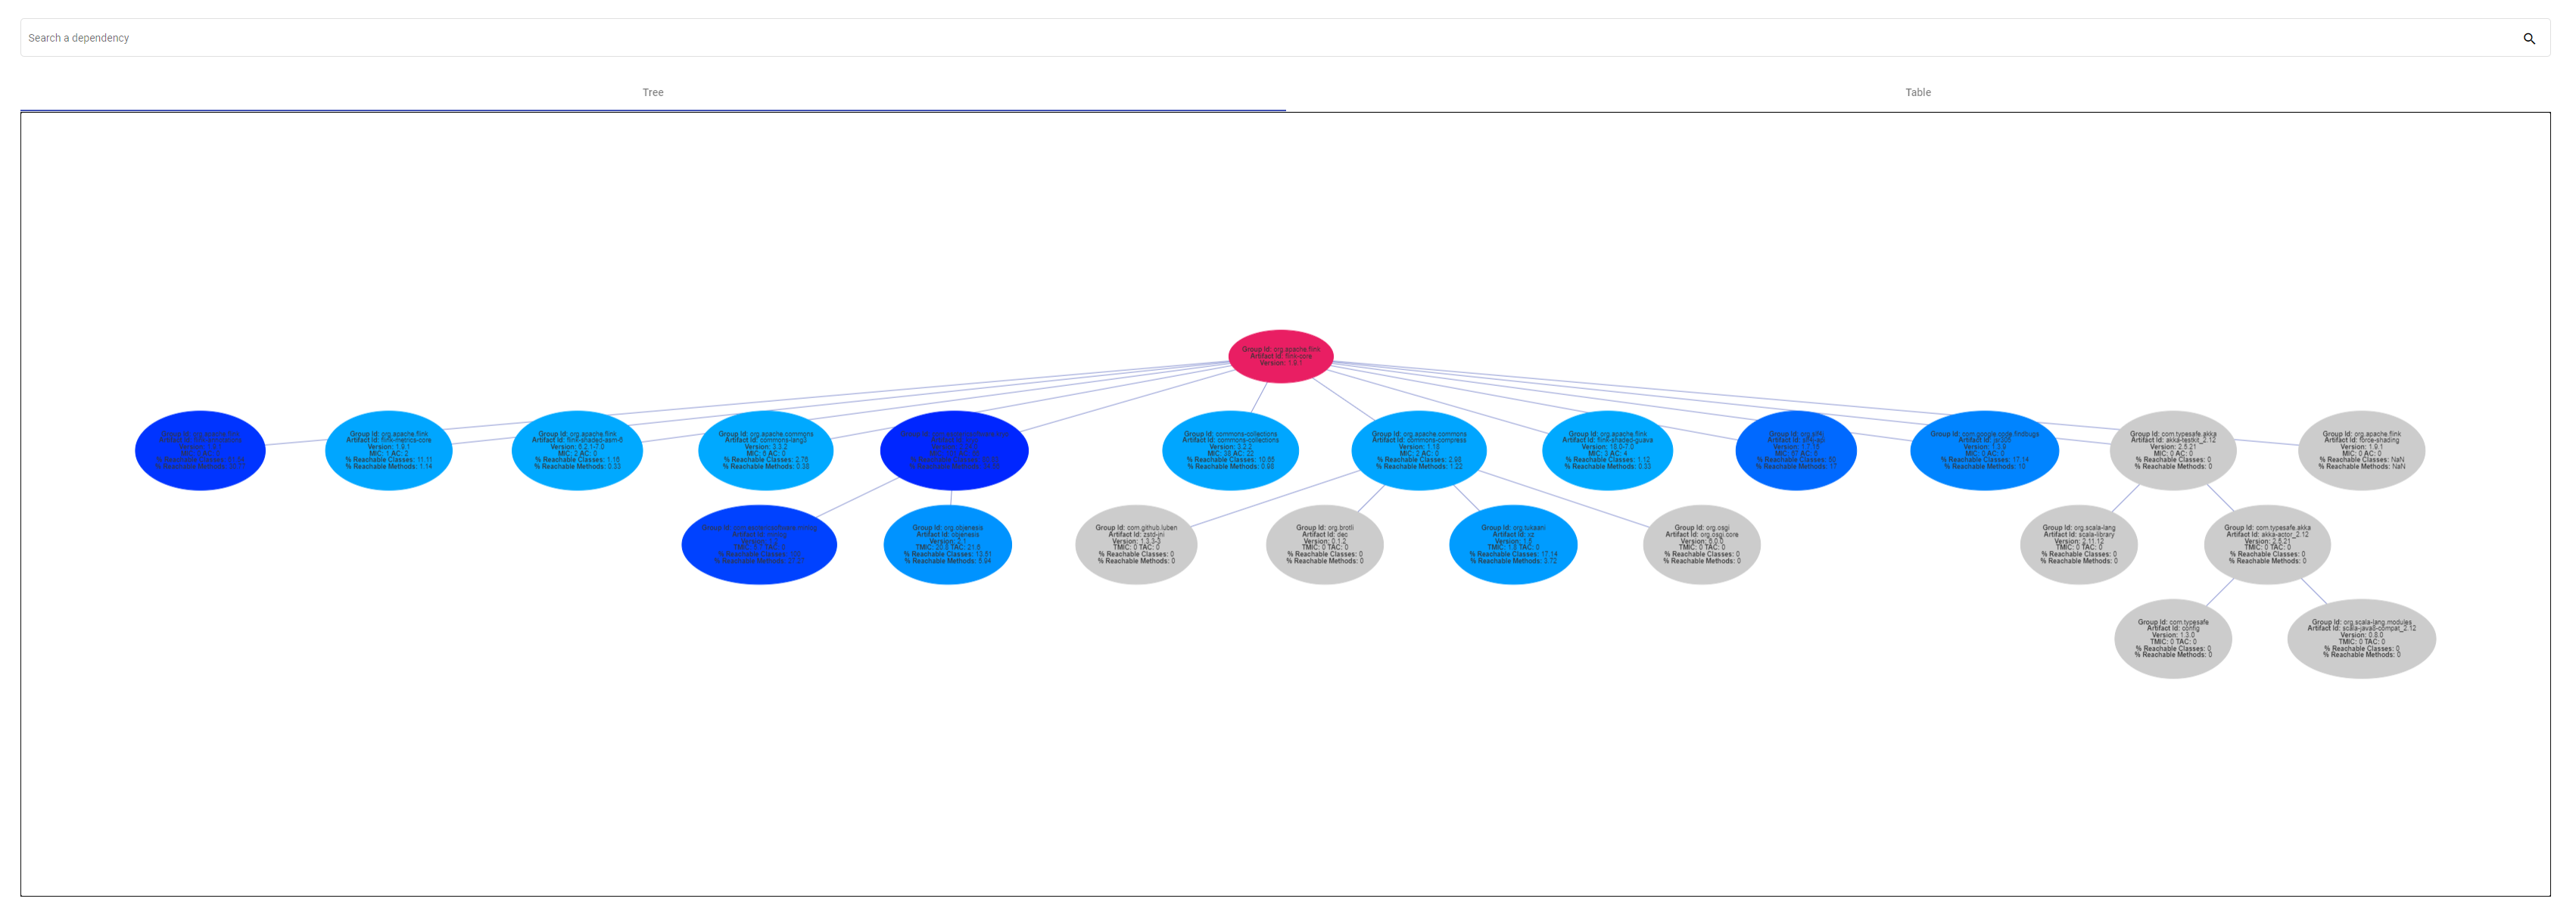
\includegraphics[width=\textwidth]{figures/tree-visualization.png}
\caption{Example of the tree visualization}
\label{fig:tree-visualization}
\end{center}
\end{figure}

\paragraph{Layout}
Since this visualization displays the dependency tree of the client library, the chosen layout is a \textit{graph}. In particular, it is a \textit{tree}. In this graph, each node represents a library, and each edge a dependency between the nodes. The tree is organized by levels, such that the first level only contains the client library, and the second level the direct dependencies. The rest of the levels are organized according to the dependencies of the previous levels.

Each node displays the following information about the library: \texttt{GroupID}, \texttt{ArtifactID}, \texttt{version}, and the result of the metrics - \texttt{MIC} and \texttt{AC} for the direct dependencies, as well as \texttt{TMIC} and \texttt{TAC} for the transitive dependencies.

\paragraph{Shape}
For this visualization, the shape of each of the nodes is the same, an ellipse. This is because the differentiation between the nodes is done with the node's color, not the shape. Furthermore, the ellipse is the shape that allows us to display all the necessary information in the node, without taking too much extra space.

\paragraph{Color}
To indicate the state of the dependency with the nodes' color, we have used three different colors. The nodes representing libraries for which no coverage has been found are light grey. Then, the rest of the dependencies have different blue shades, going from lighter blue for the less used, and darker blue for the most used. Furthermore, the color of the node representing the client library is dark pink. Finally, when a node is selected (see next paragraph), the color of the node changes to light pink.

\paragraph{Interaction}
The main problem with the dependency tree visualization is that if the tree contains too many nodes, it is very difficult to see the nodes' content. To fix this, all the nodes can be selected. When a node is selected, the visualization zooms in the selected node so that the user can see the content.

There are two ways to select a node. The first one is by clicking the node. The second option is by finding the node in the search bar. The search bar has been implemented to give suggestions containing all the libraries' names displayed in the tree. To clear the node selection, the user has to click in the graph view, outside of the nodes.

The second type of interaction has been implemented to display some additional information on the nodes. When a user hovers over a node, a \textit{tooltip} appears. The \textit{tooltip} contains the data of the library and the value of the coupling and coverage metrics. For the coupling metrics, two tables are displaying, for each metric, the value measured, and the distance at which the value was measured.

\subsection{Dependency Table}
The dependency tree visualization gives an overview of the dependencies. However, it is not useful to compare the values of the metrics among dependencies. Therefore, this second visualization is focused on seeing together all the values to sort and compare. Figure \ref{fig:table-visualization} shows the table visualization for the client library \textit{org.apache.flink:flink-core:1.9.1}.

\begin{figure}[ht]
\begin{center}
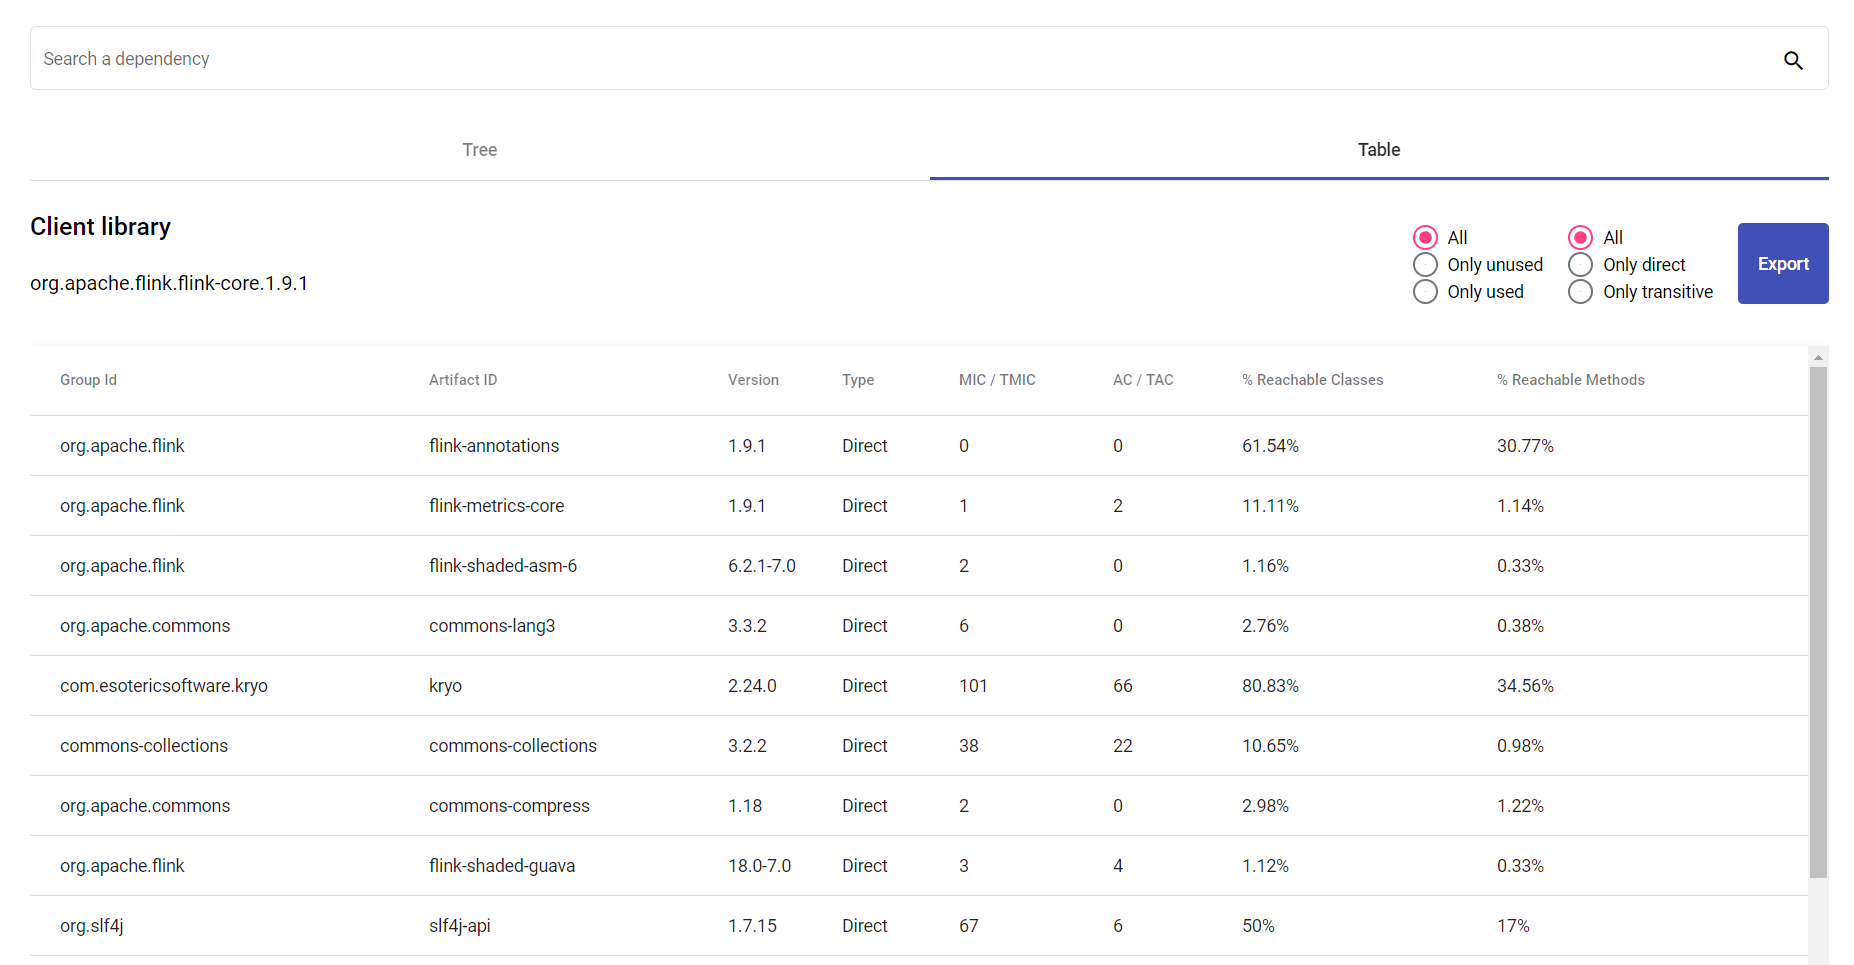
\includegraphics[width=\textwidth]{figures/table-visualization.png}
\caption{Example of the table visualization}
\label{fig:table-visualization}
\end{center}
\end{figure}

\paragraph{Layout}
To be easy to compare the value of the metrics among all the dependencies, the layout chosen for this visualization is a table. The table displays one dependency on each row, while the columns display information about the dependency, and the coupling and coverage metrics calculated for the dependency. For each library, there is a column for the \textit{groupId}, the \textit{artifactId}, the \textit{version}, and whether the dependency is direct or transitive. Then, the rest of the columns the values displayed are \texttt{MIC} and \texttt{AC} (or \texttt{TMIC} and \texttt{TAC} for transitive dependencies), and the metrics \texttt{\%ReachableClasses} and \texttt{\%ReachableMethods}.

\paragraph{Shape}
For this visualization, the shape is already defined by the layout, which is a table.

\paragraph{Color}
The color is used in this visualization only to indicate which library has been selected by the user, in which case the row of the library has a pink background. The rest of the rows have a white background.

\paragraph{Interaction}
As explained earlier, this visualization is meant to compare the values easier, and therefore the first interaction implemented for this visualization is sorting. The rows of the table can be sorted according to the values of any of the columns. Also, it is possible to filter the content of the table. The rows can be filtered based on whether the dependencies are direct or transitive, and if the client library uses the dependencies or not.

\subsection{Distribution per class}
With the previous visualizations, the user has an overview of the dependency tree. However, there is no way the user can have more detailed information about a specific library of the dependency tree. Therefore, and making use of the node selection implemented in the visualization described in section \ref{sec:visualization-dependency-tree}, we have created a visualization to display the usage per class metrics for the analyzed client library, and the selected server library. An example of this visualization for the client library \textit{org.apache.flink:flink-core:1.9.1} and the server library \textit{com.esotericsoftware.kryo:kryo:2.24.0}, can be found in Figure \ref{fig:per-class-visualization}.

\begin{figure}[ht]
\begin{center}
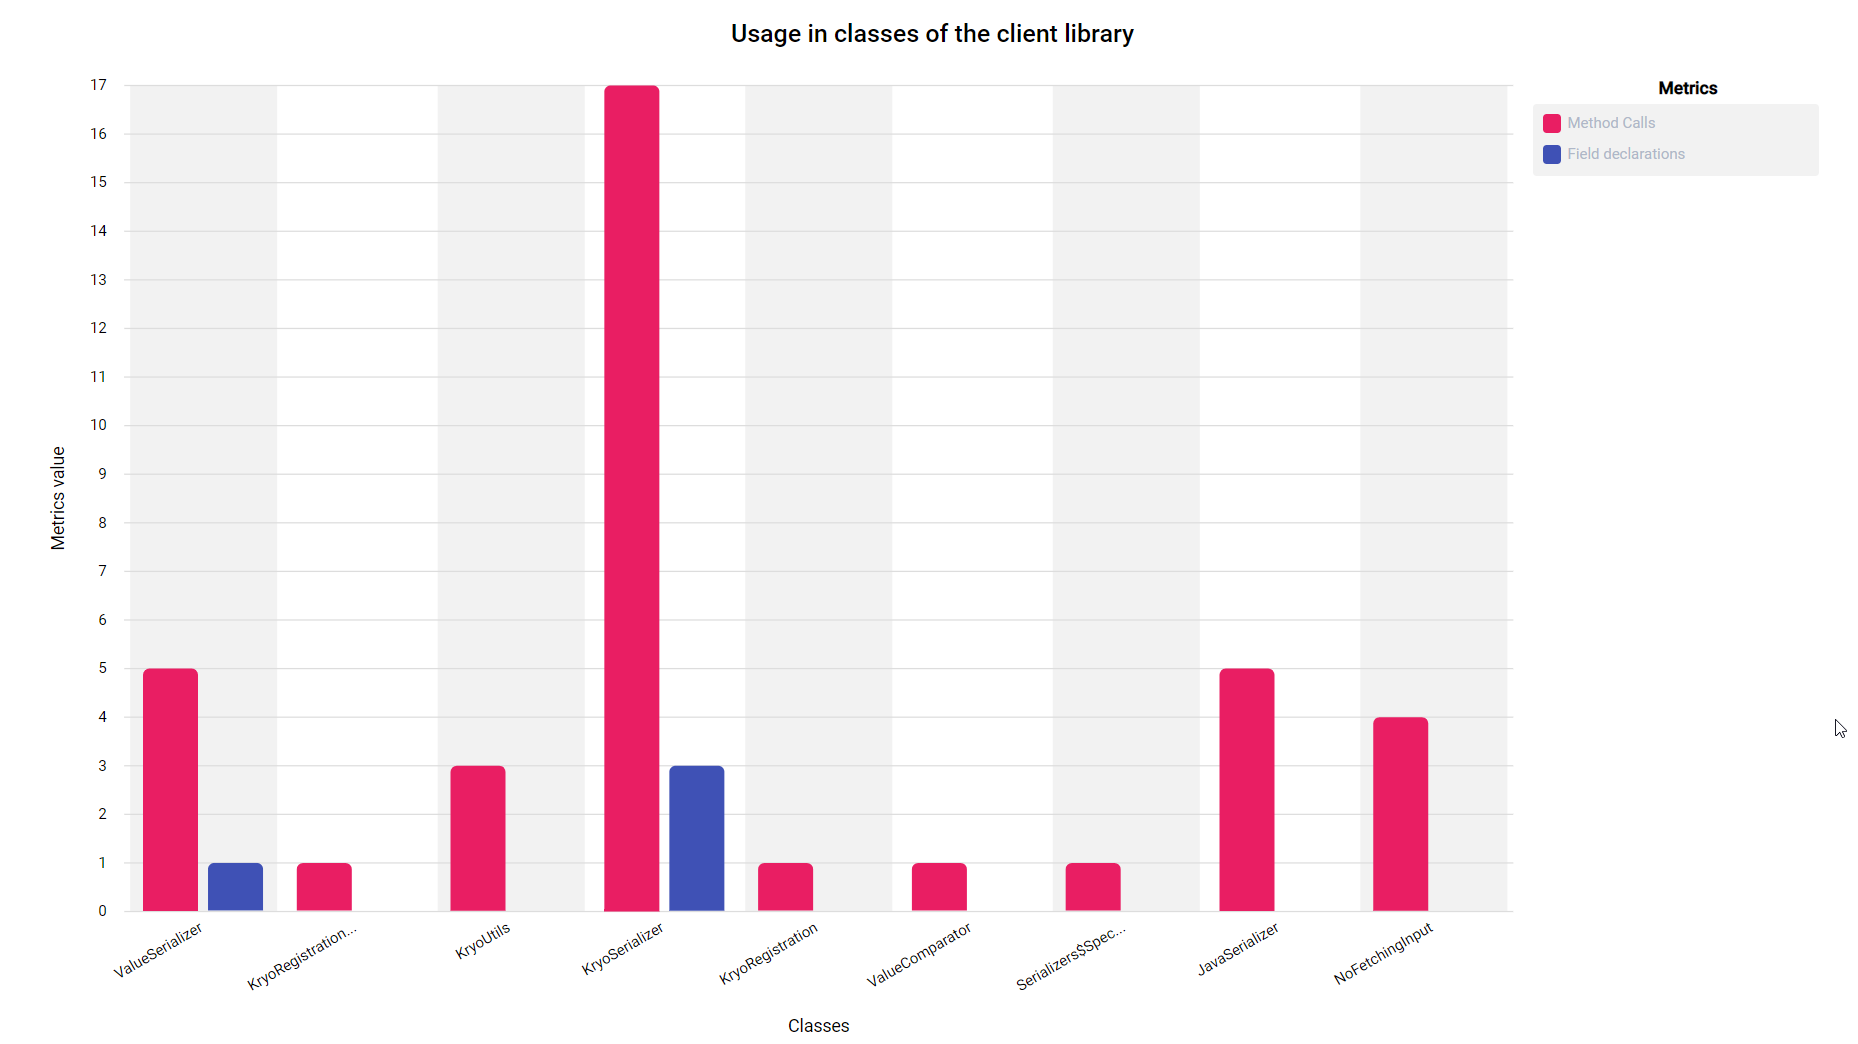
\includegraphics[width=\textwidth]{figures/per-class-visualization.png}
\caption{Example of the distribution per class visualization}
\label{fig:per-class-visualization}
\end{center}
\end{figure}

\paragraph{Layout}
The chosen layout for this visualization is a multi-chart. The chart contains two values for each represented class, the metrics \(\verb|#MethodInvocations|\) and \(\verb|#FieldDeclarations|\).
Only the classes for which at least one of the two metrics is measured appear in the chart.

\paragraph{Shape}
The shape chosen for this chart is the bar. The line was discarded since it is not the goal to show progression between the different classes. Hence, the chart used is a multi-bar chart.
At the x-axis of the chart, only the simple names of the classes are displayed to avoid having too much text in the chart. In the y-axis, there is a numeric scale, which corresponds to the calculated \(\verb|#MethodInvocations|\) and \(\verb|#FieldDeclarations|\).

\paragraph{Color}
To follow the palette used for the rest of this tool's frontend, we use the dark blue color for the bars displaying the metric \(\verb|#MethodInvocations|\), while the bars displaying the \(\verb|#FieldDeclarations|\) are pink.

\paragraph{Interaction}
This visualization appears and disappears according to the node selection of the dependency tree and table visualizations.

Also, if the user hovers the cursor over a column, a \textit{tooltip} appears. This \textit{tooltip} contains the values of the calculated metrics since these values are not displayed in the chart. In addition, it also contains the fully-qualified name of the class, to indicate the user the exact path to find the class within the project.
